\section{Results}

The model performed better than using the average
recipe in predicting the U.S. \gls{UNF}, without
a significant increase in computational time.

\subsection{Depletion Calculation Time and File Size}
For 100 random sets of
burnup and enrichment depletion calculations,
the model takes 0.27 seconds, while
searching the database for a assemblies
with the closest burnup and enrichment (using Pandas)
takes 21.8 seconds. Comparatively, 100 \gls{ORIGEN} calculations
take 118 seconds. Also, the standalone model pickle file is only
38 Kb, while the curated database (.csv) itself is 330 Mb.

\subsection{Assembly Comparison}

Ten data points were picked at random from the \gls{UDB},
and were compared with the model predictions, to observe
two things:
\begin{enumerate}
    \item What isotope (or Z, A range) the model is good / bad
        at predicting
    \item What burnup / enrichment range the model is good / bad
        at predicting
\end{enumerate}

Figures \ref{fig:3-2_29998-0}, \ref{fig:3-81_35883-0},
\ref{fig:4-0_35195-0}, and \ref{fig:4-47_50105-0}
show that the model
generally has a high relative error percentage for Ra-226
(average concentration 6.0 e-12\%), Ac-227 (average concentration  2.3 e-12\%), and curium isotopes.
The absolute prediction errors are quite small
(averaging 1e-11), but the large percent errors are due
to the small value of the data. There was not a notable
difference in the error values for enrichment
and burnup variations.

\begin{figure}
    \centering
    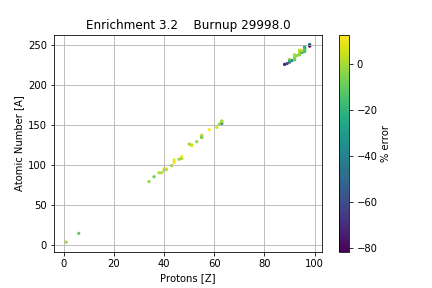
\includegraphics[width=\textwidth]{3-2_29998-0.png}
    \caption{Isotope by isotope prediction error percentage
             plotted for a discrete burnup and enrichment.}
    \label{fig:3-2_29998-0}
\end{figure}

\begin{figure}
    \centering
    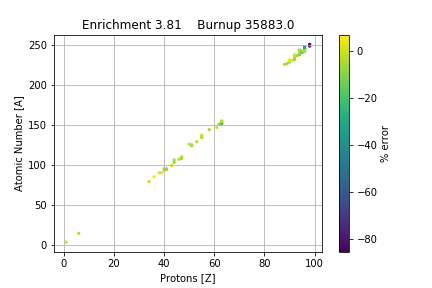
\includegraphics[width=\textwidth]{3-81_35883-0.png}
    \caption{Isotope by isotope prediction error percentage
             plotted for a discrete burnup and enrichment.
             }
    \label{fig:3-81_35883-0}
\end{figure}

\begin{figure}
    \centering
    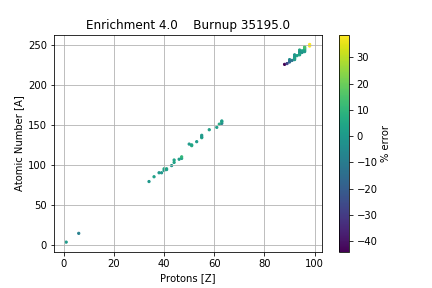
\includegraphics[width=\textwidth]{4-0_35195-0.png}
    \caption{Isotope by isotope prediction error percentage
             plotted for a discrete burnup and enrichment.
             }
    \label{fig:4-0_35195-0}
\end{figure}


\begin{figure}
    \centering
    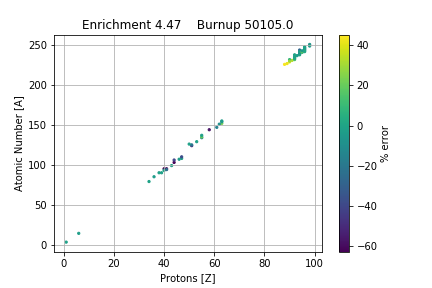
\includegraphics[width=\textwidth]{4-47_50105-0.png}
    \caption{Isotope by isotope prediction error percentage
             plotted for a discrete burnup and enrichment.
             }
    \label{fig:4-47_50105-0}
\end{figure}


\subsection{U.S. \gls{UNF} Inventory Comparison}

In this section, we compare three \gls{UNF} inventories.
The inventories are acquired by using the assembly mass and discharge date data
in the \gls{UDB}. The only difference is the composition of the
assemblies. The three different inventories acquire the composition by:

\begin{enumerate}
    \item Data: simply importing from database
    \item Prediction: model prediction of composition using burnup and enrichment from database
    \item Recipe: using an single composition (recipe) for all assemblies
\end{enumerate}

The assembly with the median burnup and assembly has an initial enrichment
of 3.85 (wt\%) and a burnup of $41,552$ MWd/MT. The concentrations of major
isotopes in the assembly are in table \ref{tab:avg_assem}.


\begin{table}[h]
    \centering
    \begin{tabular}{|l|r|r|r|r|r|}
        \hline
        Isotopes & U-235 & U-238 & Pu-239 & Cs-137 & Sr-90 \\
        \hline
        Concentration [wt\%] & 1.076 & 92.66 & 0.77 & 0.14 & 0.061 \\
        \hline
    \end{tabular}
    \caption{Isotopic concentration of the assembly with median burnup and
             enrichment. This composition is used for the recipe method. 
    \label{tab:avg_assem}}
\end{table}


We compare the three inventories on the three
metrics:
\begin{enumerate}
    \item Isotopic inventory
    \item Waste metrics (activity and decay heat)
    \item Equivalent fissile inventory (equivalent Pu-239)
\end{enumerate}

The Unified database contains discharged assembly data
from nuclear reactors in the United States up to May of
2013. We added all the \gls{UNF} assemblies in the database,
and evaluated the inventory in 2013. The results are shown
in table \ref{tab:met}.

\begin{table}[h]
    \centering
    \begin{tabular}{l|r|rr}
        \hline
        Metric & Data & Recipe & Prediction \\
        \hline
        $^{239}Pu$ mass [t] & 320.37 & 351.70 & 321.38\\
        $^{137}Cs$ mass [t] & 63.84 & 66.64 & 63.73 \\
        $^{235}U$ mass [t] & 464.60 & 487.94 & 474.14\\
        $^{238}U$ mass [t] & 42,171 & 42,016 & 42,162\\
        \hline
        Decay Heat [MW] & 193.39 & 198.55 & 193.33 \\
        Activity [Bq] & $2.79e21$ & $2.84e21$ & $2.75e21$ \\
        \hline
    \end{tabular}
    \caption{Comparison of \gls{PWR} \gls{UNF} inventory in the U.S. 
    \label{tab:met}}
\end{table}

\FloatBarrier

\subsubsection{Isotope Inventory}

Comparing the isotope inventory, the model outperforms the
average recipe method for all isotopes.
Figure \ref{fig:iso_rel} shows the relative
error between the full database, model prediction, and
the average recipe for
major isotopes. For plutonium isotopes, the model far
outperforms the average database.

\begin{figure}
    \centering
    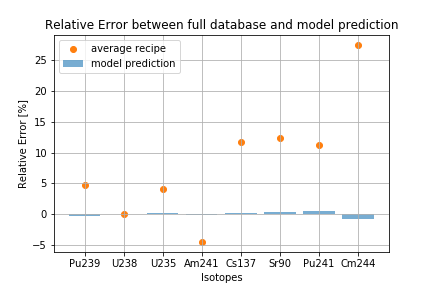
\includegraphics[width=\textwidth]{iso_rel.png}
    \caption{Relative error percentage of important isotopes}
    \label{fig:iso_rel}
\end{figure}


\begin{figure}
    \centering
    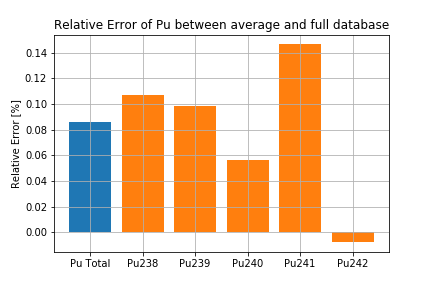
\includegraphics[width=\textwidth]{pu_rel.png}
    \caption{Relative error percentage for plutonium isotopes.}
    \label{fig:pu_rel}
\end{figure}

\FloatBarrier


\subsubsection{Waste Metric}
The model excellently predicts waste metrics activity
and decay heat. Figures \ref{fig:assem_dh} and \ref{fig:assem_act}
show the relative error percent of the decay heat and activity
predictions per assembly. The model predicts most assemblies
with an error of less than 1\%, except for assemblies with low
burnup and high enrichment.


\begin{figure}
    \centering
    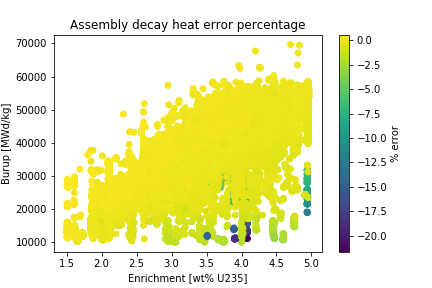
\includegraphics[width=\textwidth]{assem_dh.png}
    \caption{Relative error percentage for predicting the decay
             heat of individual assemblies.}
    \label{fig:assem_dh}
\end{figure}


\begin{figure}
    \centering
    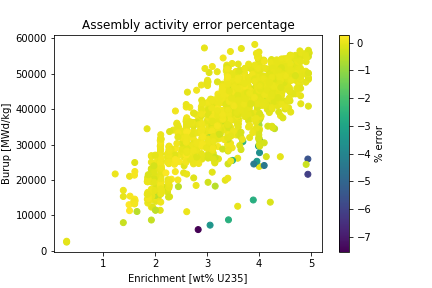
\includegraphics[width=\textwidth]{assem_act.png}
    \caption{Relative error percentage for predicting the
             activity of individual assemblies.}
    \label{fig:assem_act}
\end{figure}


Figures \ref{fig:assem_dh_recipe} and
\ref{fig:assem_act_recipe} show the relative error percent
of the decay heat and activity from the average recipe.
As shown the error is higher as the point gets farther from
the average burnup and enrichment.



\begin{figure}
    \centering
    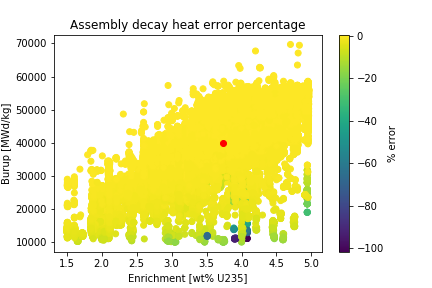
\includegraphics[width=\textwidth]{assem_dh_recipe.png}
    \caption{Relative error percentage for decay heat
             of the average recipe
             method. The red point is the average enrichment and
             burnup.}
    \label{fig:assem_dh_recipe}
\end{figure}

\begin{figure}
    \centering
    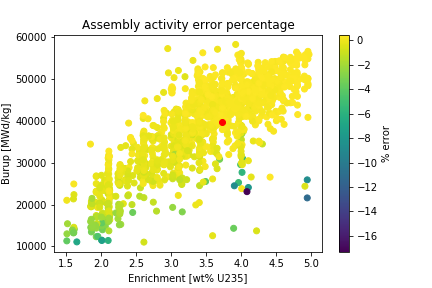
\includegraphics[width=\textwidth]{assem_act_recipe.png}
    \caption{Relative error percentage for activity
             of the assembly of the average recipe
             method. The red point is the average enrichment and
             burnup.}
    \label{fig:assem_act_recipe}
\end{figure}

\FloatBarrier


Table \ref{tab:wm} shows the decay heat and activity value
comparison in the years 2020, 2100, and 3100. The total
error is less than 1.1\% for all metrics at all time periods.
Figure \ref{fig:ha_err} shows the relative error percentage
of activity and decay heat progression in time. It shows
that the model outperforms the average recipe method
in predicting waste metrics.


\begin{table}[h]
    \centering
    \begin{tabular}{lcrrr}
        \hline
        Metric & Year & Data & Prediction  & Error [\%] \\
        \hline
        \multirow{3}{*}{\shortstack{Decay \\ Heat}} & 2020 & 40.97 & 41.07 & -0.24 \\
                                                    & 2100 & 16.42 & 16.47 & -0.35 \\
                                                    & 3100 & 3.13 & 3.14 & -0.15 \\
        \hline
        \multirow{3}{*}{\shortstack{Activity}} & 2020 & 4.67e20 & 4.66e20 & 0.21 \\
                                               & 2100 & 6.39e19 & 6.38e19 & 0.07 \\
                                               & 3100 & 3.68e18 & 3.68e18 & -0.17 \\
        \hline
    \end{tabular}
    \caption{Decay heat and radioactivity values and errors for years 2020, 2100, and 3100.}
    \label{tab:wm}
\end{table}

\begin{figure}
    \centering
    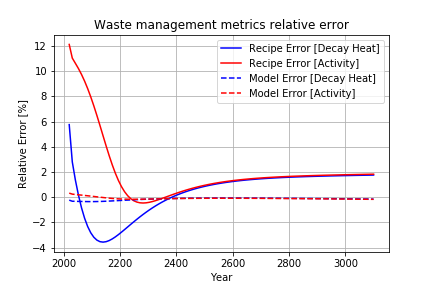
\includegraphics[width=\textwidth]{ha_err.png}
    \caption{Relative error of waste management metrics for \gls{UNF} inventory
             generated by the average recipe, and the prediction model.}
    \label{fig:ha_err}
\end{figure}

\FloatBarrier

\subsubsection{Assembly fissile quality}

Fissile quality is calculated as a metric called
equivalent plutonium-239, shown in figure \ref{fig:pu_equiv} \cite{anon_plutonium_1989}. This value is
calculated by aggregating the weighted fissile
values of each isotope in a \gls{UNF}.
For example, the equivalent fissile value for
an \gls{LWR} will be calculated by:
\begin{equation}
\text{Pu}_{eq} = 0.8(U_{235}) - (\text{Pu}_{238}) + (\text{Pu}_{239}) - 0.4(\text{Pu}_{240}) \\
            + 1.3(\text{Pu}_{241}) - 1.4(\text{Pu}_{242}) - 2.2(\text{Am}_{241})
\end{equation}
Where the variables represent the mass of each isotope.


\begin{figure}
    \centering
    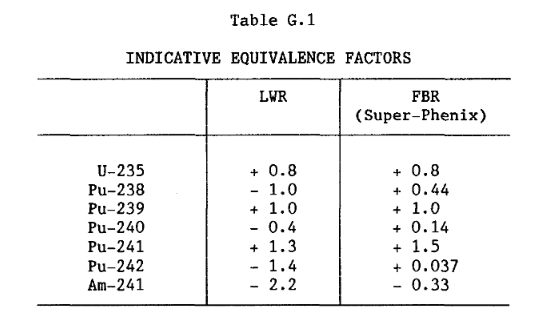
\includegraphics[width=\textwidth]{pu_equiv.png}
    \caption{Equivalent factors of each isotope for
             calculating equivalent Pu-239 value,
             from \cite{anon_plutonium_1989}. Factors
             are separated by reactor neutron spectrum
             due to cross section variations in different
             spectra.}
    \label{fig:pu_equiv}
\end{figure}

Figure \ref{fig:fiss} shows the fast equivalent Pu-239
value of the \gls{UNF} inventory plotted over time.
The trained model outperforms the recipe method. The
initial falls for all three lines are due to the
decay of plutonium 241, which has a half-life of
14 years.

\begin{figure}
    \centering
    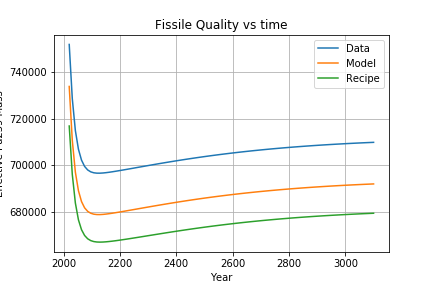
\includegraphics[width=\textwidth]{fiss.png}
    \caption{fast factors were used}
    \label{fig:fiss}
\end{figure}




\subsection{\Cyclus implementation}

Implementing the model into \Cyclus allows a 
reactor model where reactor parameters like discharge
burnup, initial enrichment, cycle time, and power
capacity is dynamic and customizable.

The created archetype in \Cyclus allows users to define
equations instead of numbers for reactor parameters.
The user can define an enrichment-burnup matrix for
each assembly in each batch, and the burnup and enrichment
values can be equations in time. This way, users can
implement reactor facilities where the reactor parameters
change in time.

Figures \ref{fig:cyclus_pu}
and \ref{fig:cyclus_fp} show the discharge fuel composition
of a reactor facility where we increased the discharge burnup
from 33,000 to 71,710 MWd/MT over 25 discharge cycles.
It should be noted that the model does not take into account
the plausibility of such fuel depletion. For example, it
would be nearly impossible for a  \gls{PWR} to burn 2\%
enriched \gls{UOX} fuel to 70,000 MWd/MT.

The user can also define dynamic
cycle time and refueling time for the reactor model, as shown
in figure \ref{fig:cyclus_time}.



\begin{figure}
    \centering
    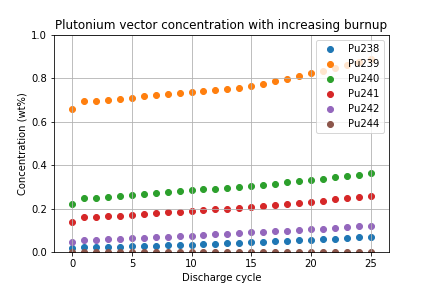
\includegraphics[width=\textwidth]{./cyclus_imp/pu.png}
    \caption{Plutonium isotope concentration in discharge fuel over discharge cycle. The model errors if the target burnup
    is over the burnup listed in the training dataset.}
    \label{fig:cyclus_pu}
\end{figure}


\begin{figure}
    \centering
    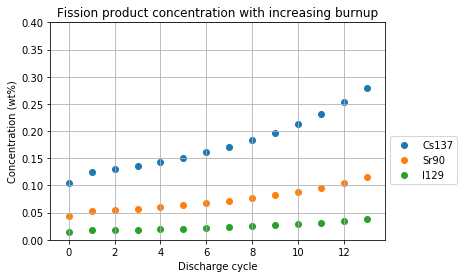
\includegraphics[width=\textwidth]{./cyclus_imp/fp.png}
    \caption{Fission product concentration in discharge fuel over discharge cycle. Increased discharge burnup leads to higher fission product concentration.}
    \label{fig:cyclus_fp}
\end{figure}

\begin{figure}
    \centering
    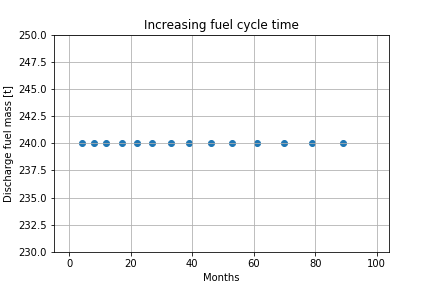
\includegraphics[width=\textwidth]{./cyclus_imp/cycle_time.png}
    \caption{Discharge and refueling cycles can be defined as an equation of time in this reactor archetype.}
    \label{fig:cyclus_time}
\end{figure}

\subsubsection{Applications and Use Cases}

The capability to set dynamic reactor parameters
allow simulation of various future transition scenarios
that depend on \gls{UNF} inventory characteristics,
such as \gls{MA} inventory. 
Users can simulate future scenarios where the discharge
burnup of reactors increases over time, and how that
affects the \gls{MA} inventory, and how that affects
transition speed. 

Also, users can simulate potential
power uprates in currently existing fleets, and
estimate how that affects \gls{UNF} inventory. With
advances in materials, reactors will have longer
cycle times and higher fuel discharge burnups.
This dynamic reactor model will be able to account
for the changes in these reactor parameters.

\FloatBarrier